\section{知识图谱构建与系统实现}
\subsection{知识图谱总体架构设计}
项目总体架构包括数据层、预处理层、术语层、抽取层、图谱层、服务层和展示层。数据层负责文献与中间结果管理；预处理层负责文本清洗与分句；术语层负责候选术语生成和 LLM 定稿；抽取层负责实体关系抽取；图谱层负责节点、边和多格式导出；服务层通过 FastAPI 提供接口；展示层基于 ECharts 进行交互可视化。

从实现思想上看，该架构并不是简单的脚本堆叠，而是典型的流水线式工程组织。每一层都以标准化文件作为输入输出边界：例如预处理层输出句子级语料，术语层输出定稿术语表，抽取层输出实体与关系记录，图谱层输出节点和边集合。这种层次化拆分使得系统具备良好的可维护性与可复现实验能力。若某一阶段策略发生变化，如术语筛选阈值调整或关系触发词补充，仅需重跑局部阶段即可，无需完全从头执行全部流程。

同时，该架构兼顾了课程项目场景下的展示需求与技术扩展性。一方面，当前系统可直接依赖本地文件运行，无需预先搭建复杂数据库环境，降低了部署门槛；另一方面，图谱层保留 JSON、CSV 与 TTL 等标准导出格式，为后续接入图数据库、RDF 推理框架或问答系统提供了接口基础。因此，这一总体架构既满足了原型系统快速实现的现实要求，也为未来扩展留出了清晰空间。

\subsection{实体抽取与关系抽取实现}
实体识别以 \texttt{terms\_final.csv} 为词典基础，辅以规则识别部分参数类与结构类实体。关系抽取则采用“同句实体对—触发词匹配—约束过滤—三元组输出”的流程。项目引入触发词位置约束、实体黑名单、距离阈值和实体类型约束四重过滤机制，显著提高了关系抽取的精度。

在实体抽取阶段，系统重点解决的是“高召回识别”与“实体边界稳定”之间的平衡问题。若词典过小，则容易遗漏大量领域术语；若词典过大，则容易引入噪声概念。因此项目先通过术语构建阶段尽量扩大候选覆盖，再在抽取阶段通过最长匹配、重叠消解和类型校验抑制误识别。例如，较长的专业术语在匹配时具有更高优先级，以避免短词将长词切碎；同时，对明显缺乏领域意义的黑名单词项进行过滤，以减少通用词误判为实体的现象。

在关系抽取阶段，系统强调“可解释规则优先”与“大语言模型增强”相结合的双模理念。对于具有金标准的明确术语，系统通过显式触发词模式定义候选关系类型，再结合实体类型兼容性、实体间最大距离和句内位置顺序进行过滤，保证抽取的高度可解释性。为了弥补纯规则抽取带来的图谱稀疏（“散点图”）问题，系统在降级模式下引入了基于大模型的上下文感知三元组抽取。该模块将包含多个候选实体的长难句进行动态批处理（每批约 200 条），并通过 \texttt{ThreadPoolExecutor} 开启多达 8 个并发工作线程。这种并行计算架构不仅大幅缩短了处理耗时，更凭借 LLM 的语义理解能力有效覆盖了规则难以处理的隐式关联。

\begin{figure}[H]\centering
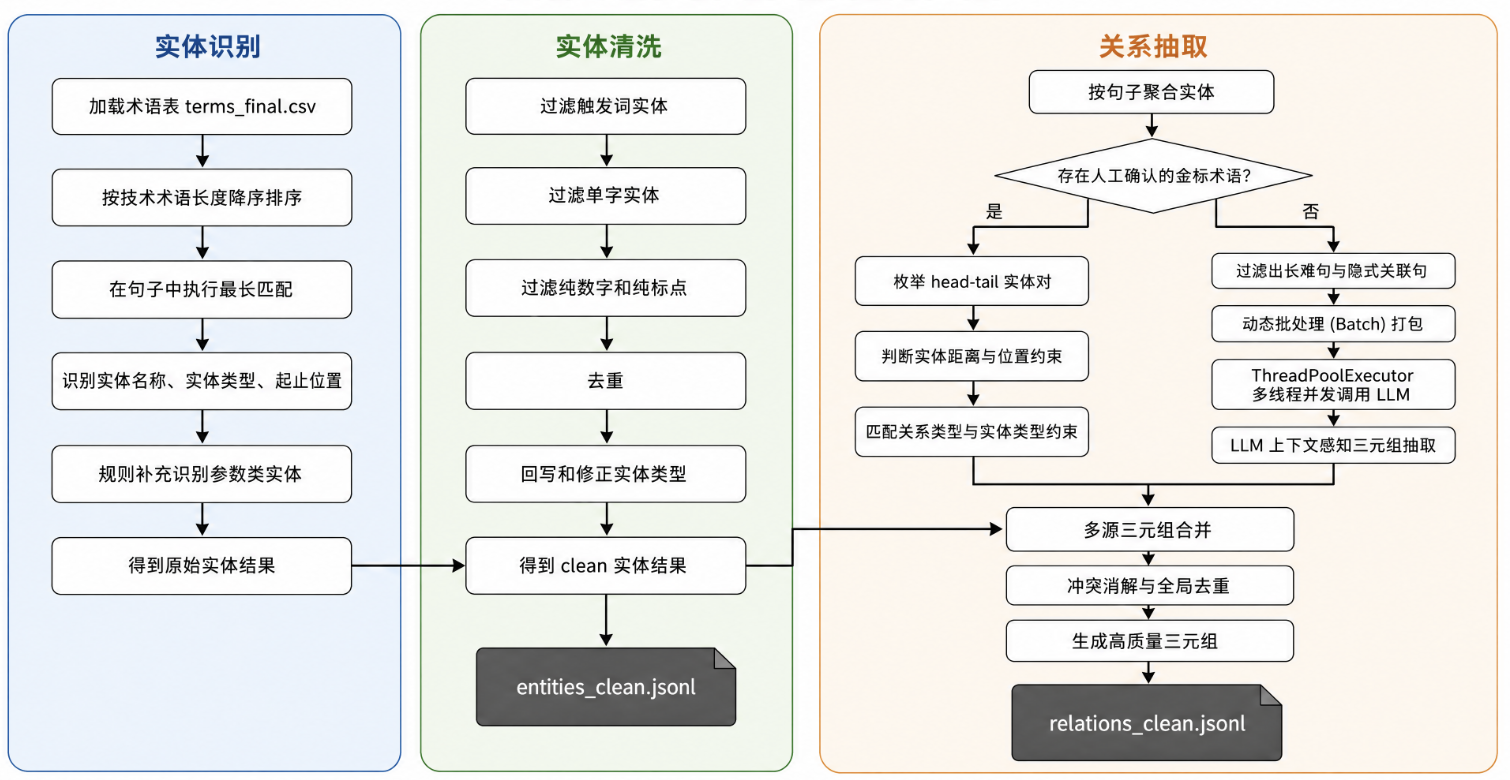
\includegraphics[width=1\textwidth]{figures/实体识别与关系抽取流程图.png}
\caption{实体识别与关系抽取流程图}
\end{figure}

\begin{lstlisting}[style=pythonstyle,caption={关系抽取约束示意}]
RELATION_PATTERNS = [
    ("is_a", ["是一种", "属于", "可视为"]),
    ("has_component", ["包括", "包含", "组成"]),
]
MAX_ENTITY_DISTANCE = 80
\end{lstlisting}

\subsection{图谱数据导出与存储}
图谱构建模块将实体与关系组织为节点集和边集，并导出为 \texttt{kg.json}、\texttt{nodes.csv}、\texttt{edges.csv} 和 \texttt{kg.ttl}。其中 \texttt{kg.json} 直接供前端使用，CSV 便于图数据库导入，TTL 便于 RDF 语义表达。这样的多格式导出方式体现了较强的规范性和扩展性。

在导出阶段，系统并不是简单地将抽取结果原样写出，而是先进行节点去重、名称标准化和关系重组，再根据不同使用场景输出不同格式的数据文件。图~\ref{fig:export} 展示了这一过程，有助于说明图谱结果如何从抽取记录转化为可展示、可分析、可复用的结构化图谱数据。

\begin{figure}[H]\centering
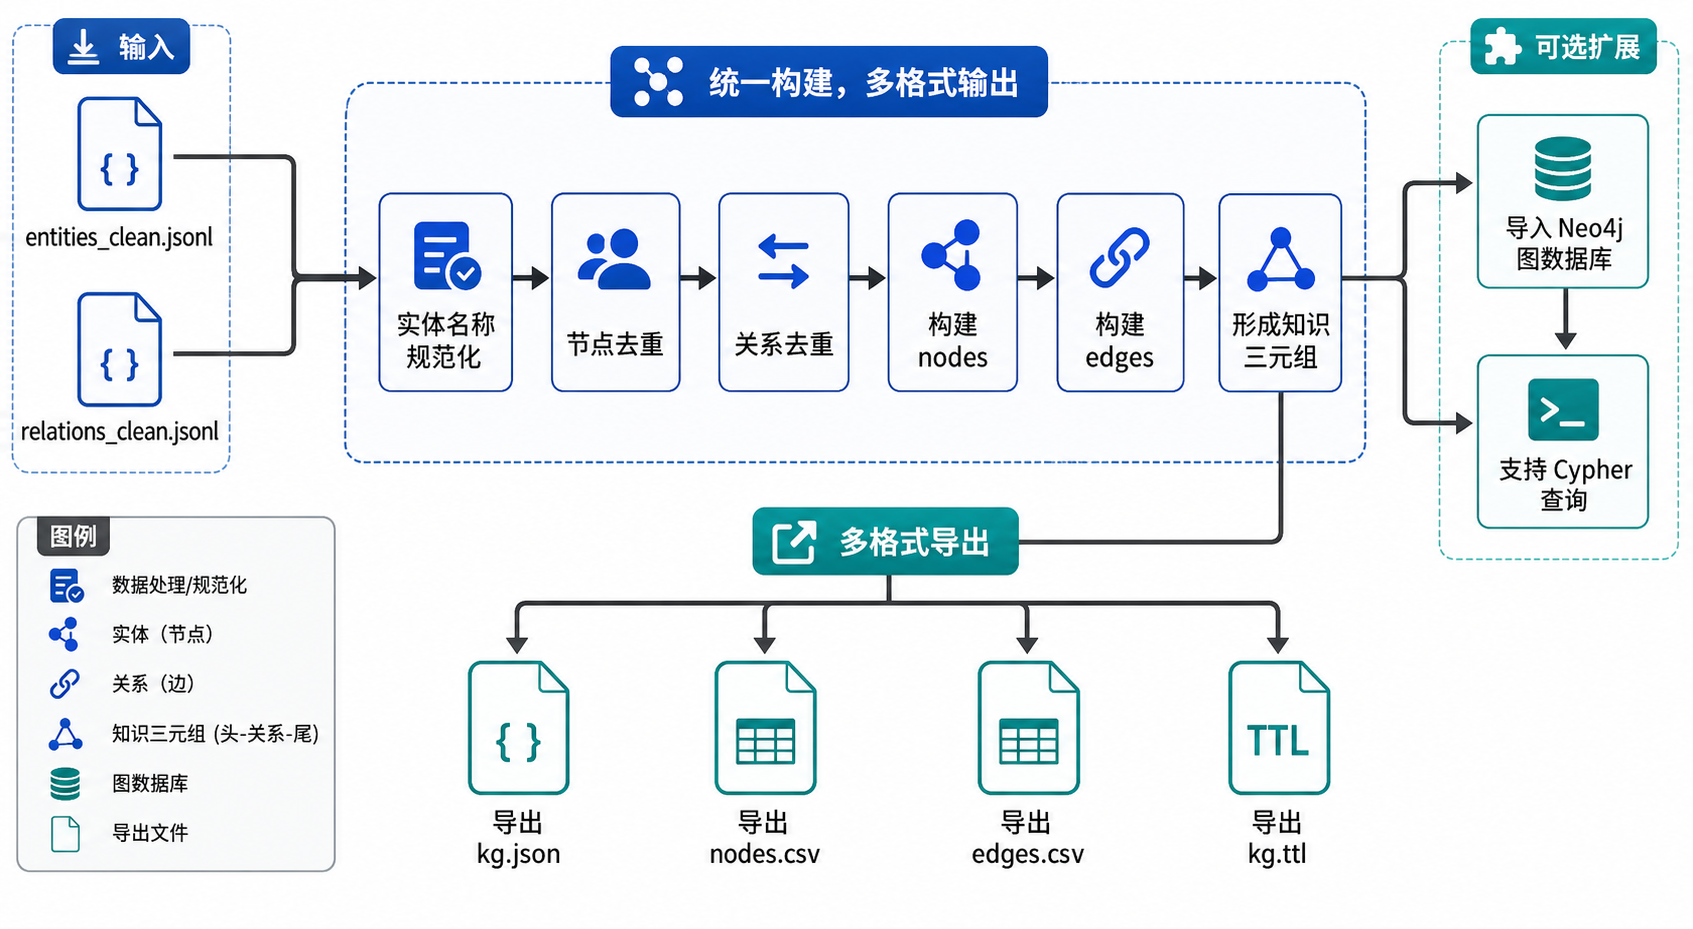
\includegraphics[width=0.86\textwidth]{figures/知识图谱构建与多格式导出流程图.png}
\caption{知识图谱构建与多格式导出流程图}
\label{fig:export}
\end{figure}

\subsection{知识图谱可视化系统实现}
项目使用 FastAPI + ECharts 构建了轻量级前后端一体化图谱系统。后端直接加载 \texttt{kg.json} 即可运行，避免了答辩环境中必须部署图数据库的复杂性；前端支持图谱总览、实体搜索、类型筛选、实体详情展示与局部子图钻取，使图谱不仅可以被看到，还可以被解释和分析。

在后端实现上，系统将图谱统计、搜索、节点详情和中心子图等功能封装为独立接口，从而使前端页面逻辑与底层数据组织方式解耦。这样做的好处在于：一方面可以让前端专注于交互与展示，另一方面也便于后续将文件型图谱替换为数据库型图谱而不必完全重写前端逻辑。在前端实现上，力导向图被用作主要展示形式，是因为它更适合呈现实体之间的聚类关系、中心节点和局部连接强度，有助于用户从视觉上快速把握图谱结构。

此外，系统在可视化层面并非仅追求“好看”，而是尽量服务于知识探索任务。实体搜索帮助用户快速定位目标概念；类型筛选帮助用户隔离不同语义层次的节点；实体详情面板帮助用户查看节点属性与关联边；局部子图则帮助用户以某个中心实体为起点展开邻域分析。在交互体验优化方面，前端重构了关键操作的确认逻辑，通过自定义异步 Modal 对话框替换了原生 \texttt{window.confirm}，彻底解决了大规模并行构建任务中浏览器 UI 线程被阻塞的缺陷。通过这些功能，图谱由静态结果图转化为流畅可交互的知识组织界面，这也是本项目的重要实现特点之一。

图~\ref{fig:main-ui} 展示了系统主界面。该界面主要用于呈现知识图谱整体分布、节点聚类状态以及全局交互效果，是用户进入系统后最先接触到的总览页面。通过主界面，用户可以先形成对图谱规模、结构和热点实体的整体认识，再进一步进行局部探索。

\begin{figure}[H]\centering
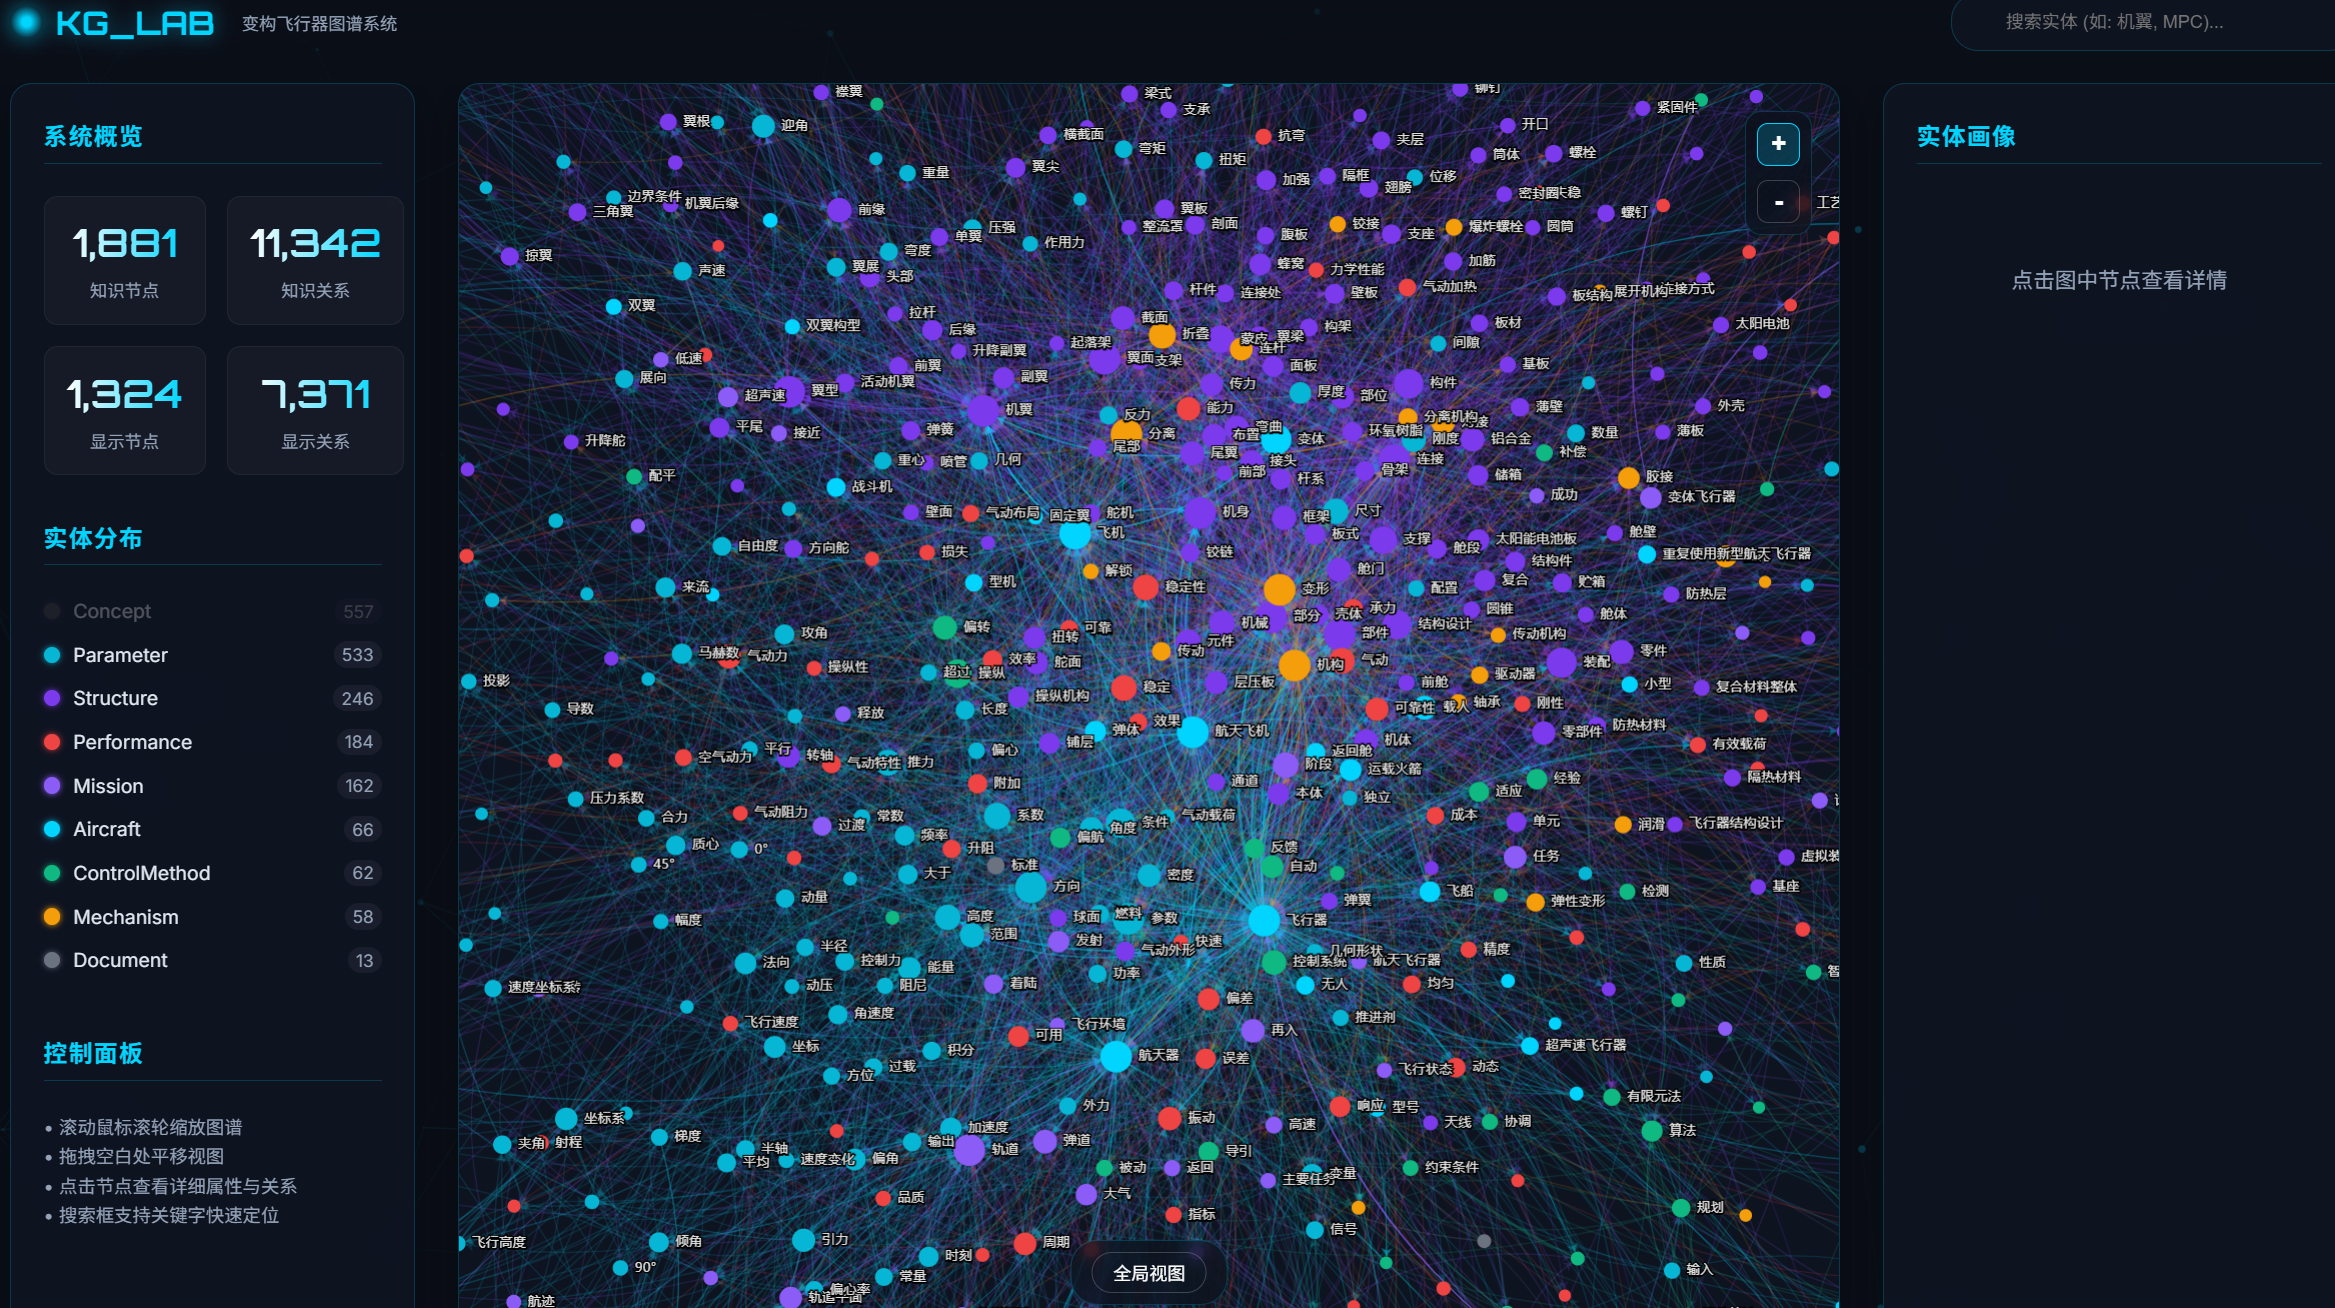
\includegraphics[width=0.90\textwidth]{figures/前端整体展示图.png}
\caption{知识图谱可视化系统主界面}
\label{fig:main-ui}
\end{figure}

在完成整体浏览后，用户还需要查看单个实体的属性信息及其周边关系。图~\ref{fig:detail-ui} 展示了实体详情与关联关系展示界面，该界面能够将中心实体的基本信息、关联节点和对应关系同步呈现，便于分析某一概念在图谱中的语义位置与关联范围。

\begin{figure}[H]\centering
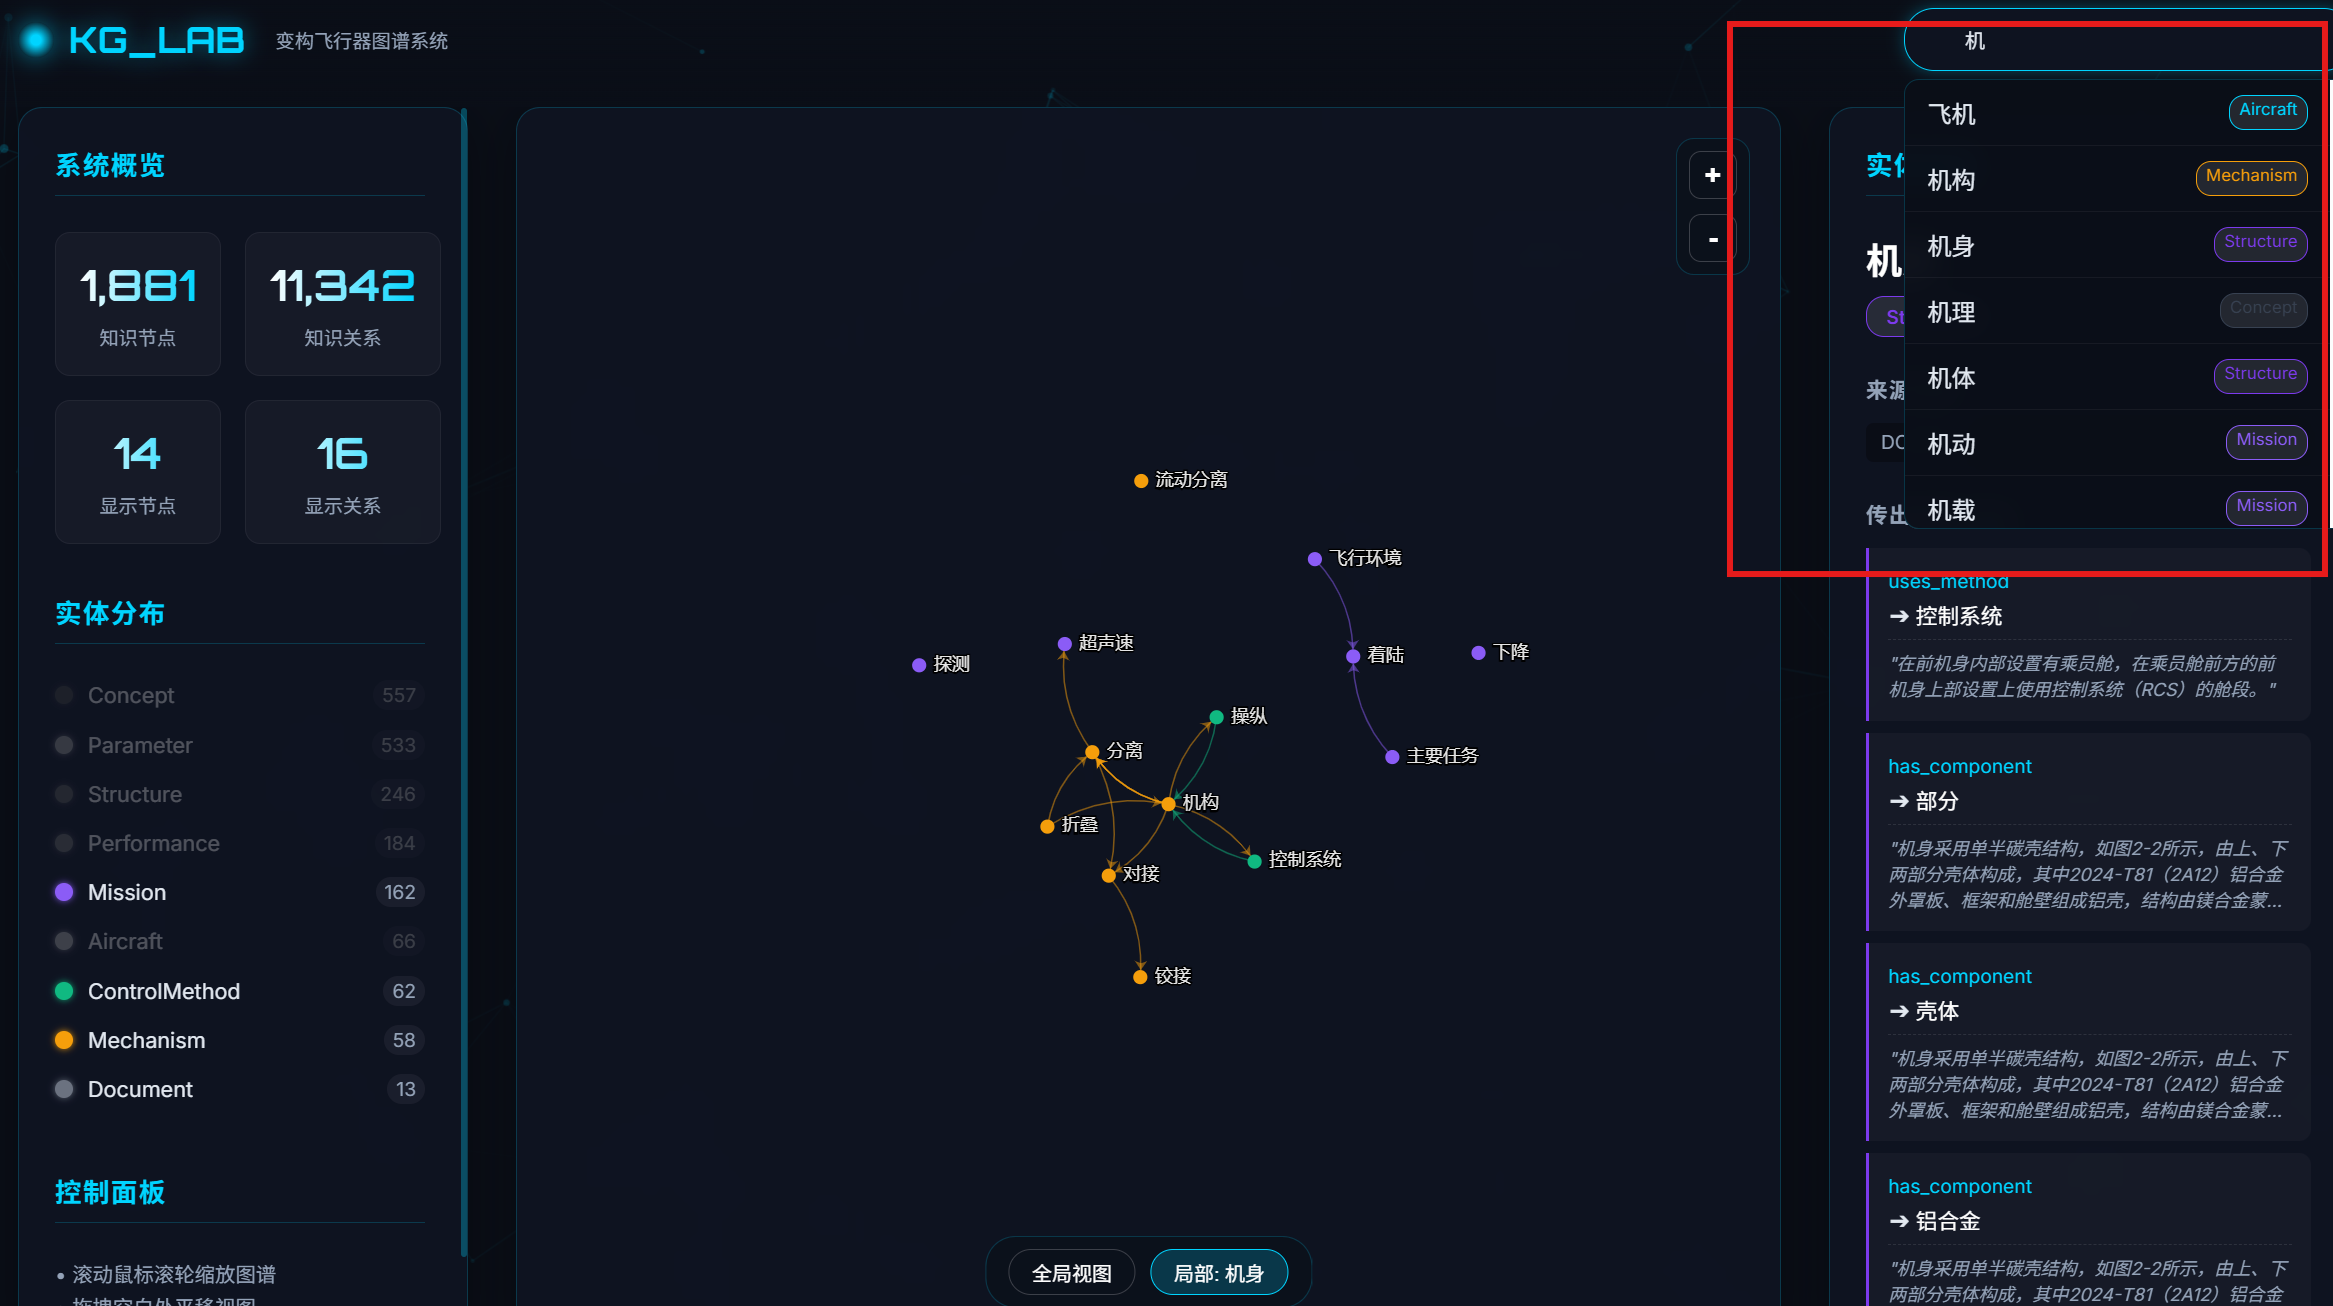
\includegraphics[width=0.9\textwidth]{figures/实体详情与关联关系展示界面.png}
\caption{实体详情与关联关系展示界面}
\label{fig:detail-ui}
\end{figure}

当用户希望从更高层次理解图谱中不同类型实体的分布结构时，类型筛选功能就变得尤为重要。图~\ref{fig:filter-ui} 展示了基于实体类型筛选的图谱显示效果。通过对不同实体类别进行过滤，用户可以更清晰地观察某一类节点的聚合形态及其与其他类型节点之间的连接模式，从而提高图谱分析的针对性。

\begin{figure}[H]\centering
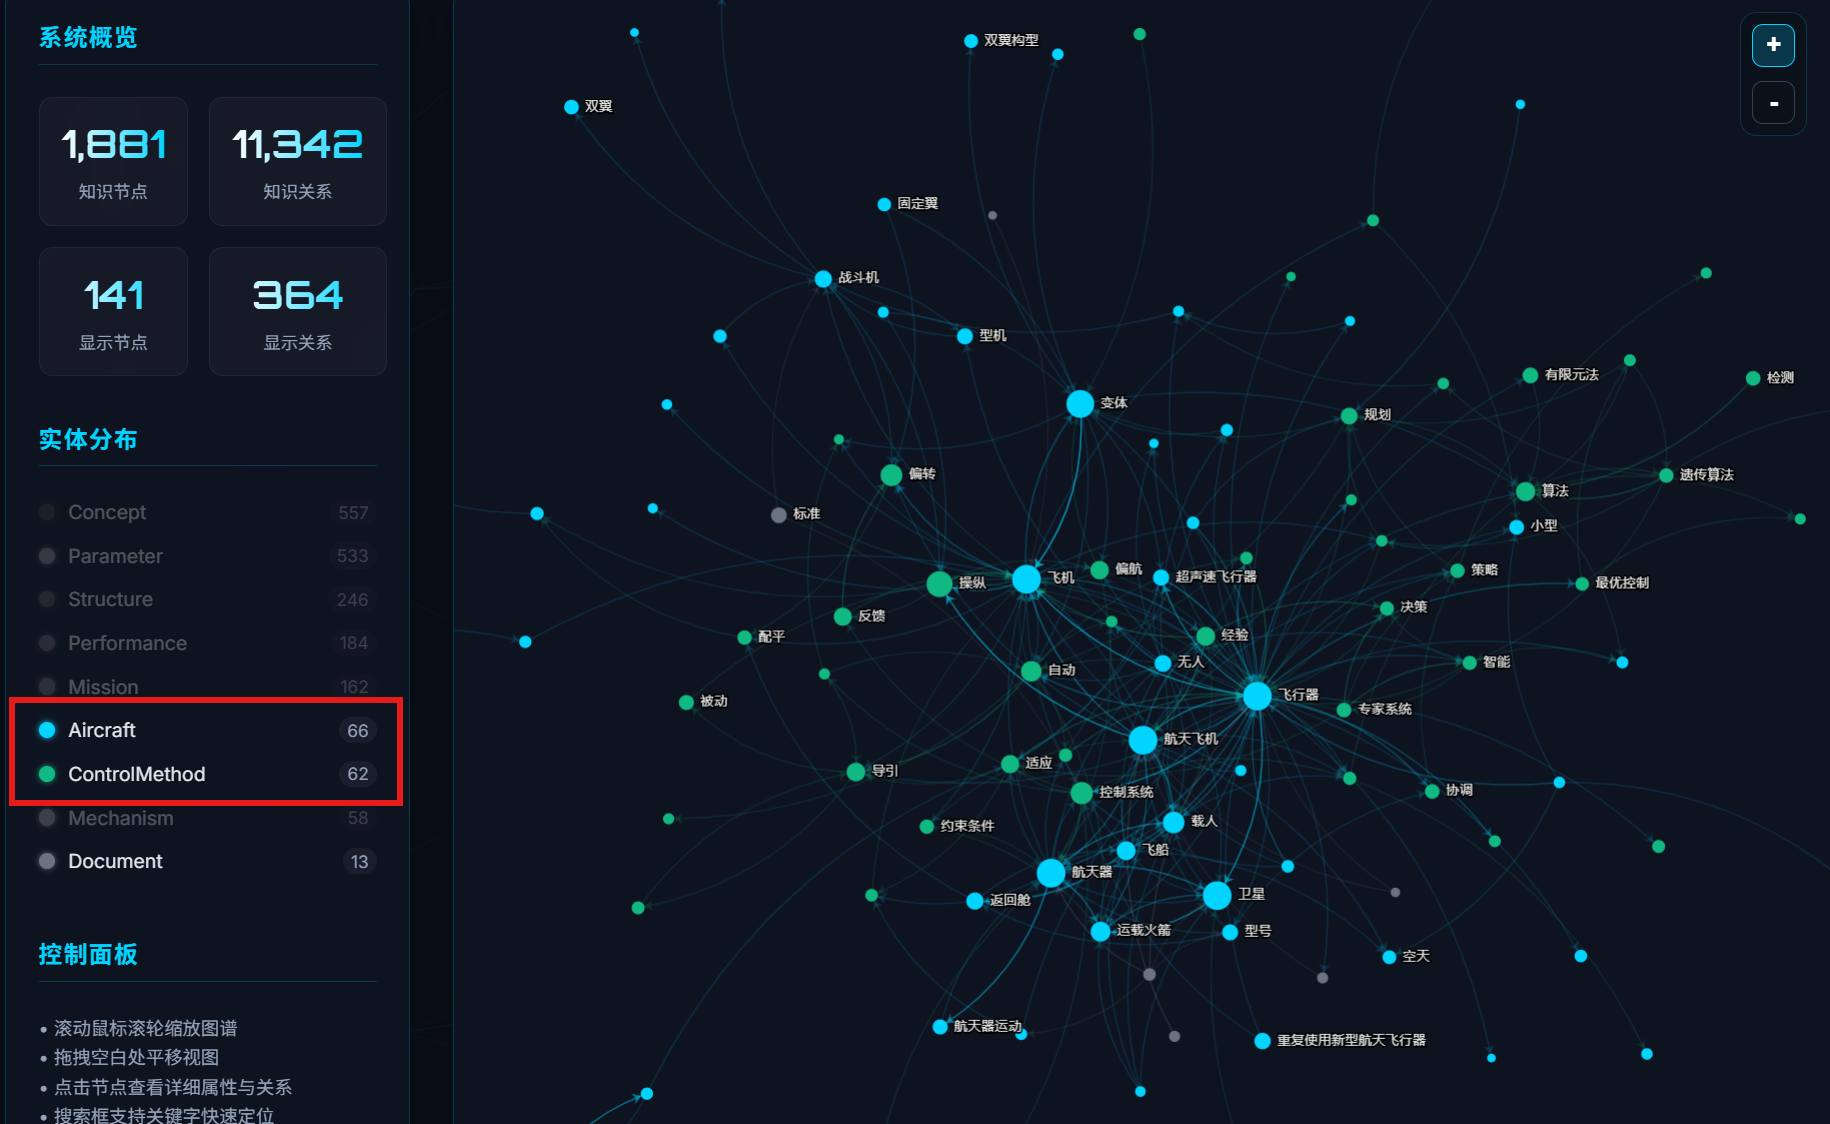
\includegraphics[width=0.9\textwidth]{figures/基于实体类型筛选的图谱显示效果.png}
\caption{基于实体类型筛选的图谱显示效果}
\label{fig:filter-ui}
\end{figure}
